\documentclass[8pt]{beamer}

\newif\ifplacelogo % create a new conditional
\placelogotrue % set it to true

\usetheme{Warsaw}
\usecolortheme{rose}
\usepackage{multicol}
\usepackage{epstopdf}
\usepackage[italic]{hepnames}
\usepackage{tikz}
\usepackage{listings}
\usepackage{times}
\usepackage{amsmath}
\usepackage{verbatim}
\usepackage{hyperref}
\usepackage{bbding}
\usepackage{gensymb}
\usepackage{upgreek}
\lstset{breakatwhitespace,
language=C++,
columns=fullflexible,
keepspaces,
breaklines,
tabsize=3, 
showstringspaces=false,
extendedchars=true}

% TikZ includes!!!
\usepackage{tikz}
\usetikzlibrary{backgrounds}
\usetikzlibrary{calc}
\tikzstyle{every picture}+=[remember picture]
\input{/home/oviazlo/Desktop/beamerPresentations/myReports/latexHelpScripts/tikzGrid.tex}


\begin{document}

% custom colors
\definecolor{olive}{rgb}{0.3, 0.4, .1}
\definecolor{fore}{RGB}{249,242,215}
\definecolor{back}{RGB}{51,51,51}
\definecolor{title}{RGB}{255,0,90}
\definecolor{dgreen}{rgb}{0.,0.6,0.}
\definecolor{gold}{rgb}{1.,0.84,0.}
\definecolor{JungleGreen}{cmyk}{0.99,0,0.52,0}
\definecolor{BlueGreen}{cmyk}{0.85,0,0.33,0}
\definecolor{RawSienna}{cmyk}{0,0.72,1,0.45}
\definecolor{Magenta}{cmyk}{0,1,0,0}

\definecolor{PixelColor}{RGB}{207,232,139}
\definecolor{SCTColor}{RGB}{167,166,255}
\definecolor{TRTColor}{RGB}{250,224,140}
\definecolor{grayColor}{RGB}{153,153,153}

\newcommand{\yRefPosOne}{0.0}
\newcommand{\xRefPosOne}{0.0}
\newcommand{\yRefPosTwo}{0.0}
\newcommand{\xRefPosTwo}{0.0}
\newcommand{\yRefIncrementOne}{0.0}
\newcommand{\xRefIncrementOne}{0.0}
\newcommand{\yRefIncrementTwo}{0.0}
\newcommand{\xRefIncrementTwo}{0.0}

\graphicspath{ {/home/oviazlo/Desktop/beamerPresentations/FCCee/pictures/2018_jul25/} }


\DeclareGraphicsExtensions{.eps, .pdf, .png}

\newcommand{\myBox}[2][pink] {
    \noindent\colorbox{#1}{
	\textbf{#2}
    }\par
}

% For nice block (provided by Oleh)
\tikzstyle{myBox} = [draw=red, fill=blue!1, very thick,
    rectangle, rounded corners, inner sep=5pt, inner ysep=9pt]
    
\tikzstyle{PixelBox} = [draw=PixelColor, fill=blue!1, very thick,
    rectangle, rounded corners, inner sep=5pt, inner ysep=9pt]
\tikzstyle{SCTBox} = [draw=SCTColor, fill=blue!1, very thick,
    rectangle, rounded corners, inner sep=5pt, inner ysep=9pt]
\tikzstyle{TRTBox} = [draw=TRTColor, fill=blue!1, very thick,
    rectangle, rounded corners, inner sep=5pt, inner ysep=9pt]

% poster advertisement
\newcommand{\myCenterBox}[2][pink] {
   {\centering
    \noindent\colorbox{#1}{
	\textbf{#2}
    }\par
  }
}

\newcommand{\mySmallCenterBox}[2][pink] {
   {\centering
    \noindent\colorbox{#1}{
	\textbf{{\small #2}}
    }\par
  }
}

\newcommand{\myVerySmallCenterBox}[2][pink] {
   {\centering
    \noindent\colorbox{#1}{
	\textbf{{\scriptsize #2}}
    }\par
  }
}

\newcommand{\backupbegin}{
   \newcounter{finalframe}
   \setcounter{finalframe}{\value{framenumber}}
}
\newcommand{\backupend}{
   \setcounter{framenumber}{\value{finalframe}}
}

\newcommand{\myNode}{\tikz[baseline,inner sep=1pt] \node[anchor=base]}

\tikzstyle{fancytitle} =[fill=white!15, text=black]

\definecolor{light-gray}{gray}{0.95}
% poster advertisement


\title[Calorimetry performance with CLD \hspace{14.0em}\insertframenumber/
\inserttotalframenumber]{Contribution of the incoherent pairs background to the calorimeter system}


	\author[Oleksandr Viazlo]{Oleksandr Viazlo\\ 
	{\small }
	}
	\institute{\small CERN\\} 
	
       
	\date{25 July 2018}

% 	\logo{ \ifplacelogo \includegraphics[height=1.8cm]{./ID_week2/lund_uni-logo_s.pdf} \hspace{0.4cm} \fi}

	
%    	\frame{\titlepage}

   	

\placelogofalse

%*****************************************************************************
\begin{frame}{\large \large Introduction}

\renewcommand{\yRefPosOne}{0}
\renewcommand{\xRefPosOne}{5.3}
\renewcommand{\xRefIncrementOne}{5.5}
\begin{tikzpicture}[overlay]

%  \node[inner sep=0pt] (tmp) at (\xRefPosOne-2.15,\yRefPosOne-0.56)
%     {\includegraphics[width=7.8cm]{FCCeePictsFromKonrad/CLIC_FCC_Top_QuarterView_withLabes.png}};

    
\node  at (\xRefPosOne,\yRefPosOne) (box){%
    \begin{minipage}{\textwidth}

  \begin{itemize}
   \item Study contribution of the incoherent pairs background to the calorimeter system 
      \begin{itemize} 
    \item simulate only-background events\\[0.4cm]
    \end{itemize}
   
   \item Assumed time integration window: 400 ns
   \begin{itemize} 
    \item 20BX overlaid at 91 GeV and 1BX overlay at 365 GeV\\[0.4cm]
    \end{itemize}
   
   \item Local runs (low statistic)\\[0.6cm]
   

  


  \end{itemize}

    \end{minipage}
};

% \node [PixelBox] at (\xRefPosOne+0.2,\yRefPosOne-3.5) (box){%
%   \begin{minipage}{0.85\textwidth}
%     Detector performances have been studied with full detector simulation
%   \end{minipage}
% };


%% HELPER draw advanced helping grid with axises:
% \draw(-0.5,-4) to[grid with coordinates] (11.5,4);
\end{tikzpicture}

 
\end{frame}
%*****************************************************************************

%*****************************************************************************
\begin{frame}{\large \large Calorimeter RAW energy vs. time}

\renewcommand{\yRefPosOne}{-1.5}
\renewcommand{\xRefPosOne}{5.3}
\renewcommand{\xRefIncrementOne}{5.5}
\begin{tikzpicture}[overlay]

 \node[inner sep=0pt] (tmp) at (\xRefPosOne-2.7,\yRefPosOne+2.0)
    {\includegraphics[width=6cm]{overlay_91GeV/overlay_energyVsHitTime.pdf}};
    
 \node[inner sep=0pt] (tmp) at (\xRefPosOne+3.3,\yRefPosOne+2.0)
    {\includegraphics[width=6cm]{overlay_365GeV/overlay_energyVsHitTime.pdf}};
    
   \node  at (\xRefPosOne-2.5,\yRefPosOne+4.35) (box){%
    \myCenterBox{\small 20BX at 91GeV}
    };     
    
       \node  at (\xRefPosOne+3.5,\yRefPosOne+4.35) (box){%
    \myCenterBox{\small 1BX at 365GeV}
    };     
 
 \node  at (\xRefPosOne+0.1,\yRefPosOne-1.9) (box){%
    \begin{minipage}{1.1\textwidth}
  \begin{itemize}
  \item Calorimeter RAW energy (no calibration constant applied)
  \item Background activity at 91GeV is contained within $\sim$10ns
  


    \end{itemize}
    \end{minipage}
  };

% % HELPER draw advanced helping grid with axises:
% \draw(-0.5,-4) to[grid with coordinates] (11.5,4);
\end{tikzpicture}
 
\end{frame}
%*****************************************************************************

%*****************************************************************************
\begin{frame}{\large \large Total deposited energy per subdetector }

\renewcommand{\yRefPosOne}{-1.5}
\renewcommand{\xRefPosOne}{5.3}
\renewcommand{\xRefIncrementOne}{5.5}
\begin{tikzpicture}[overlay]

 \node[inner sep=0pt] (tmp) at (\xRefPosOne-2.7,\yRefPosOne+2.0)
    {\includegraphics[width=6cm]{overlay_91GeV/overlay_totalEnergy.pdf}};
    
 \node[inner sep=0pt] (tmp) at (\xRefPosOne+3.3,\yRefPosOne+2.0)
    {\includegraphics[width=6cm]{overlay_365GeV/overlay_totalEnergy.pdf}};
    
    \node  at (\xRefPosOne-2.5,\yRefPosOne+4.35) (box){%
    \myCenterBox{\small 20BX at 91GeV}
    };     
    
       \node  at (\xRefPosOne+3.5,\yRefPosOne+4.35) (box){%
    \myCenterBox{\small 1BX at 365GeV}
    };     
 
 \node  at (\xRefPosOne+0.1,\yRefPosOne-1.9) (box){%
    \begin{minipage}{1.1\textwidth}
  \begin{itemize}
  \item Largest deposited energy from the background is observed in ECAL Endcap; lowest - in HCAL Barrel
  


    \end{itemize}
    \end{minipage}
  };

% % HELPER draw advanced helping grid with axises:
% \draw(-0.5,-4) to[grid with coordinates] (11.5,4);
\end{tikzpicture}
 
\end{frame}
%*****************************************************************************

%*****************************************************************************
\begin{frame}{\large \large Energy vs Z}

\renewcommand{\yRefPosOne}{-1.5}
\renewcommand{\xRefPosOne}{5.3}
\renewcommand{\xRefIncrementOne}{5.5}
\begin{tikzpicture}[overlay]

 \node[inner sep=0pt] (tmp) at (\xRefPosOne-2.7,\yRefPosOne+2.0)
    {\includegraphics[width=6cm]{overlay_91GeV/overlay_energyVsZ_Barrel.pdf}};
    
 \node[inner sep=0pt] (tmp) at (\xRefPosOne+3.3,\yRefPosOne+2.0)
    {\includegraphics[width=6cm]{overlay_365GeV/overlay_energyVsZ_Barrel.pdf}};
    
       \node  at (\xRefPosOne-2.5,\yRefPosOne+4.35) (box){%
    \myCenterBox{\small 20BX at 91GeV}
    };     
    
       \node  at (\xRefPosOne+3.5,\yRefPosOne+4.35) (box){%
    \myCenterBox{\small 1BX at 365GeV}
    };     
 
 \node  at (\xRefPosOne+0.1,\yRefPosOne-1.9) (box){%
    \begin{minipage}{1.1\textwidth}
  \begin{itemize}
  \item Energy deposition in the Barrel region as function of Z
  \item Negligible effect
  


    \end{itemize}
    \end{minipage}
  };

% % HELPER draw advanced helping grid with axises:
% \draw(-0.5,-4) to[grid with coordinates] (11.5,4);
\end{tikzpicture}
 
\end{frame}
%*****************************************************************************

%*****************************************************************************
\begin{frame}{\large \large Energy vs Radius}

\renewcommand{\yRefPosOne}{-1.5}
\renewcommand{\xRefPosOne}{5.3}
\renewcommand{\xRefIncrementOne}{5.5}
\begin{tikzpicture}[overlay]

 \node[inner sep=0pt] (tmp) at (\xRefPosOne-2.7,\yRefPosOne+2.0)
    {\includegraphics[width=6cm]{overlay_91GeV/overlay_energyVsRadius_Endcap.pdf}};
    
 \node[inner sep=0pt] (tmp) at (\xRefPosOne+3.3,\yRefPosOne+2.0)
    {\includegraphics[width=6cm]{overlay_365GeV/overlay_energyVsRadius_Endcap.pdf}};
    
    \node  at (\xRefPosOne-2.5,\yRefPosOne+4.35) (box){%
    \myCenterBox{\small 20BX at 91GeV}
    };     
    
       \node  at (\xRefPosOne+3.5,\yRefPosOne+4.35) (box){%
    \myCenterBox{\small 1BX at 365GeV}
    };     
 
 \node  at (\xRefPosOne+0.1,\yRefPosOne-1.9) (box){%
    \begin{minipage}{1.1\textwidth}
  \begin{itemize}
  \item Energy deposition in the Endcap region as function of Radius
  


    \end{itemize}
    \end{minipage}
  };

% % HELPER draw advanced helping grid with axises:
% \draw(-0.5,-4) to[grid with coordinates] (11.5,4);
\end{tikzpicture}
 
\end{frame}
%*****************************************************************************

%*****************************************************************************
\begin{frame}{\large \large Energy vs Radius}

\renewcommand{\yRefPosOne}{-1.5}
\renewcommand{\xRefPosOne}{5.3}
\renewcommand{\xRefIncrementOne}{5.5}
\begin{tikzpicture}[overlay]

 \node[inner sep=0pt] (tmp) at (\xRefPosOne-2.7,\yRefPosOne+2.0)
    {\includegraphics[width=6cm]{overlay_91GeV/overlay_energyVsTheta.pdf}};
    
 \node[inner sep=0pt] (tmp) at (\xRefPosOne+3.3,\yRefPosOne+2.0)
    {\includegraphics[width=6cm]{overlay_365GeV/overlay_energyVsTheta.pdf}};
    
       \node  at (\xRefPosOne-2.5,\yRefPosOne+4.35) (box){%
    \myCenterBox{\small 20BX at 91GeV}
    };     
    
       \node  at (\xRefPosOne+3.5,\yRefPosOne+4.35) (box){%
    \myCenterBox{\small 1BX at 365GeV}
    };     
 
 \node  at (\xRefPosOne+0.1,\yRefPosOne-1.9) (box){%
    \begin{minipage}{1.1\textwidth}
  \begin{itemize}
   \item Overall the energy deposition from incoherent pairs in calorimeter is not significant
  


    \end{itemize}
    \end{minipage}
  };

% % HELPER draw advanced helping grid with axises:
% \draw(-0.5,-4) to[grid with coordinates] (11.5,4);
\end{tikzpicture}
 
\end{frame}
%*****************************************************************************

\backupbegin
%*****************************************************************************
\begin{frame}
\frametitle{BACKUP} 
 
\end{frame}
%*****************************************************************************

%*****************************************************************************
\begin{frame}{\large \large CLD and CLICdet detector models}

\renewcommand{\yRefPosOne}{0}
\renewcommand{\xRefPosOne}{5.3}
\renewcommand{\xRefIncrementOne}{5.5}
\begin{tikzpicture}[overlay]

 \node[inner sep=0pt] (tmp) at (\xRefPosOne-2.15,\yRefPosOne-0.56)
    {\includegraphics[width=7.8cm]{../CALOR2018/fromPreviousTalks/FCCeePictsFromKonrad/CLIC_FCC_Top_QuarterView_withLabes.png}};

\node  at (\xRefPosOne,\yRefPosOne+2.8) (box){%
\myCenterBox{\small CLD model}
}; 
    
    \draw[black, thick, ->] (-0.8,-4.76)--(-0.8,3.7) node[pos=0.95, right]{\small R [m]};
    \draw[black, thick, ->] (-0.8,-4.76)--(6.5,-4.76) node[pos=0.95, below]{\tiny Z [m]};
    
  \node[inner sep=0pt] (tmp) at (\xRefPosOne-3.05,\yRefPosOne-4.9)
    {2.3};   
  \node[inner sep=0pt] (tmp) at (\xRefPosOne-1.14,\yRefPosOne-4.9)
    {3.7};  
    
%     \node [PixelBox] at (\xRefPosOne+3.7,\yRefPosOne-4) (box){%
%   \begin{minipage}{0.43\textwidth}
%     Detector design inspired by detectors for CLIC and ILC and optimized for FCC-ee conditions
%   \end{minipage}
% };

\node  at (\xRefPosOne+3.5,\yRefPosOne-0.7) (box){%
    \begin{minipage}{0.5\textwidth}

  \begin{itemize}
      \item Full silicon tracking system
      - provides $\geqslant$12 hits per track 
         \begin{itemize}
   
%     \item provides $\geqslant$12 hits per track 
    \item R$_{outer} = 1.5$m - CLICdet  \\
%     R$_{outer} = 2.1$m - CLD}\\
         \item R$_{outer} = 2.1$m - CLD\\
         {\color{black} \tiny increased material budget for 50$\%$ in VTX - CLD} \\[0.6cm]
    
   \end{itemize}
      
%       \\[0.6cm]
%       \item 2 T magnetic field (constraints from the machine) $\to$ 2.1 m large tracker radius \\[0.4cm]
      \item Fine-grained ECAL and HCAL optimised for particle flow reconstruction \\[0.6cm]
      \item Superconducting solenoid is outside of the calorimeters 
               \begin{itemize}
   
%     \item provides $\geqslant$12 hits per track 
    \item 4T field - CLICdet  \\
%     R$_{outer} = 2.1$m - CLD}\\
         \item 2T field - CLD\\[0.6cm]
%          {\color{black} \tiny increased material budget for 50$\%$ in VTX - CLD} \\[0.6cm]
    
   \end{itemize}
      
      
      \item Steel return yoke with muon chambers \\[-0.1cm]
         \begin{itemize}
    \item 2 m thickness - CLICdet \\
    \item  1.5 m thickness - CLD  \\[0.6cm]
   \end{itemize}
     
   
%    \item Forward detector region ($<$ 150 mrad) is reserved for Machine-Detector Interface (accommodates LumiCal)\\[0.6cm]
%    
   \item Support structures, cables and services are implemented in the simulation models
%    : \\ MDI region 
%    (accommodates LumiCal)
   \\[0.3cm]
  \end{itemize}

    \end{minipage}
};


% \node [PixelBox] at (\xRefPosOne+3.7,\yRefPosOne-4) (box){%
%   \begin{minipage}{0.43\textwidth}
%     Detector design inspired by detectors for CLIC and ILC and optimized for FCC-ee conditions
%   \end{minipage}
% };

%% HELPER draw advanced helping grid with axises:
% \draw(-0.5,-4) to[grid with coordinates] (11.5,4);
\end{tikzpicture}

 
\end{frame}
%*****************************************************************************

\backupend
%********************************************************
\end{document}

